\documentclass[a4paper, 12pt]{article}
\usepackage{graphicx}
\graphicspath{{images/}}
\usepackage{listings}
\usepackage[english]{babel}
\usepackage{caption}
\usepackage{color}
\usepackage{array}


\title{Homework 2}
\author{Nasir Mohammad Khalid}

\makeatletter
\let\thetitle\@title
\let\theauthor\@author
\let\thedate\@date
\makeatother

\definecolor{codegreen}{rgb}{0,0.6,0}
\definecolor{codegray}{rgb}{0.5,0.5,0.5}
\definecolor{codepurple}{rgb}{0.58,0,0.82}
\definecolor{backcolour}{rgb}{0.95,0.95,0.92}

\lstdefinestyle{mystyle}{
    backgroundcolor=\color{backcolour},   
    commentstyle=\color{codegreen},
    keywordstyle=\color{magenta},
    numberstyle=\tiny\color{codegray},
    stringstyle=\color{codepurple},
    basicstyle=\scriptsize,
    breakatwhitespace=false,         
    breaklines=true,                 
    captionpos=b,                    
    keepspaces=true,                 
    numbers=left,                    
    numbersep=1pt,                  
    showspaces=false,                
    showstringspaces=false,
    showtabs=false,                  
    tabsize=1
}

\lstset{style=mystyle}

\newenvironment{conditions}
  {\par\vspace{\abovedisplayskip}\noindent\begin{tabular}{>{$}l<{$} @{${}={}$} l}}
  {\end{tabular}\par\vspace{\belowdisplayskip}}

\begin{document} 
    \begin{titlepage}
        \centering
        \vspace*{0.5 cm}
        
\includegraphics[scale = 0.60]{logo.png}\\[1.0 cm]	% University Logo
        \textsc{\LARGE American University of Sharjah}\\[1.0 cm]
        \textsc{\Large ELE494-09}\\[0.2 cm]	
        \textsc{\Large Deep Networks in Machine Learning}\\[0.5 cm]			% Course Code
        \rule{\linewidth}{0.2 mm} \\[0.4 cm]
        { \huge \bfseries \thetitle}\\
        \rule{\linewidth}{0.2 mm} \\[1.5 cm]
        
        \textsc{\Large{\theauthor}}\\[0.3 cm]
        \textsc{\Large{65082}}\\[0.3 cm]
        \textsc{\Large{\thedate}}\\[1.5 cm]

        \textmd{Submitted To: \itshape{Dr.Usman Tariq}}
    \end{titlepage}

    \clearpage
    \tableofcontents
    \listoffigures
    \lstlistoflistings
    \clearpage

    \section{Task 1: Backpropagation}

    \subsection{Q1}

    The goal of this part to develop a theoretical understanding of how do you get the expressions with
    backpropagation algorithm. Suppose you have a three layer fully connected neural network (input layer,
    hidden layer and output layer). Following are some further "specifications":

    \begin{itemize}
        \item The input feature vectors are d dimensional (you can think of these as MNIST images, attened as vectors)
        \item There are N feature vectors in you training dataset
        \item There are H hidden nodes and K output nodes (for K mutually exclusive classes).
        \item This neural network is to be trained for classification under cross-entropy loss function
    \end{itemize}

    Derive the equations for batch gradient updates for the input-to-hidden unit weights and hidden-to-output
    unit weights. Is it wise to use a learning rate parameter? Why?

    \subsection{Answer}

    Based on the specifications given we can assume the architecture of the neural network to be as follows:

    \begin{figure}[h!]
        \centering
        \captionsetup{justification=centering}
        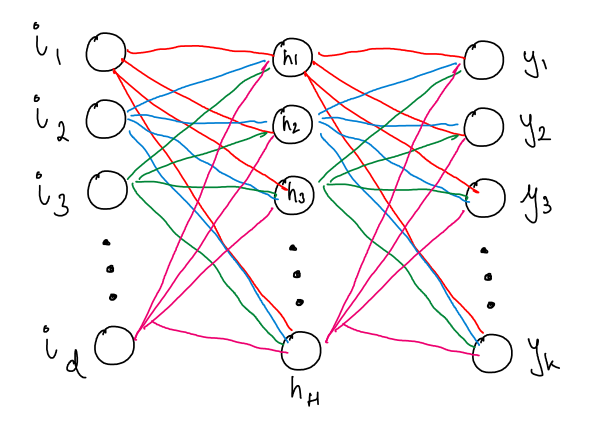
\includegraphics[scale = 0.35]{1.png}
        \caption{Representation of the neural network}
    \end{figure}
    
    The input to any one of the hidden layer nodes can be given as the sum of the bias and the product of weights and inputs. This will be as follows:

    \begin{equation}
        I_h = \sum_{n=1}^{d} i_n * w_{nh}
    \end{equation}

    where:

    \begin{center}
        \begin{conditions}
            $$I_h$$     &   Input to node h of hidden layer \\
            $$i_n$$     &   Input to node n of the input layer \\   
            $$w_{nh}$$  &   Weight between input node $$n$$ and the hidden node $$h$$\\
        \end{conditions}
    \end{center}
    
    
    Since the output consists of K mutually exclusive classes then we can take the label for the feature vectors to be of a matrix of length K
    and it contains a 1 at the appropriate label. Then the cross entropy loss function is given as:

    $$ E = - \sum_{i=1}^{k} Label_k * log(y_k) $$

    Since we are using a cross entropy loss function, we therefore assume that the outputs of the hidden layer are the result
    of a softmax function. Therefore they can be given as:

    $$ H_h = e^{\sum_{i=1}^{d} } $$




\end{document} 